% Hakuna matata | Entry 12
\begin{ArtPage}
\EntryStart
\begin{center}
{\Fontgaramondbold\fontsize{6.5}{9}\selectfont\color{Muted}ENTRY 12\par}
\vspace{0.8cm}
{\Fontgaramond\fontsize{38}{45}\selectfont\color{Ink}Hakuna matata\par}
\vspace{0.35cm}
{\Fontgaramond\fontsize{6.5}{9}\selectfont\color{Muted}%
  [hah-KOO-nah mah-TAH-tah] \enspace·\enspace EXPRESSION\par}
\vspace{0.8cm}
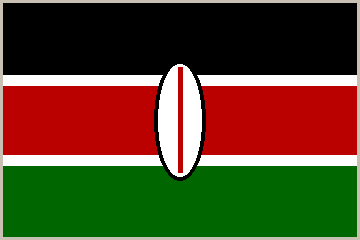
\includegraphics[height=.55cm,keepaspectratio]{assets/flags/flag_kenya.png}%
\hspace{0.5cm}%

\includegraphics[height=.55cm,keepaspectratio]{assets/flags/flag_tanzania.png}\par
\vspace{0.2cm}
{\Fontgaramond\fontsize{6.5}{9}\selectfont\color{Muted}SWAHILI / EAST AFRICA\par}
\end{center}
\EntryRuleBlock
\begin{minipage}{.92\linewidth}
\centering
{\Fontgaramond\fontsize{14}{18}\selectfont\color{Ink}%
  Literally “there are no troubles”: a reassuring expression meaning “no
  worries” or “no problem.”\par}
\end{minipage}
\EntryDefinitionGap
\begin{center}
{\Fontgaramonditalic\fontsize{17.5}{22}\selectfont\color{Poetic}%
  “To let go of what you cannot control.”\par}
\end{center}
\EntryFooterGap
\begin{center}
{\Fontgaramond\fontsize{6}{8}\selectfont\color{Muted}THE ART OF LETTING GO\par}
\vspace{0.3cm}
{\Fontgaramond\fontsize{5.5}{7}\selectfont\color{Muted}%
  THE ART OF BEING \enspace·\enspace ENTRY 12\par}
\end{center}
\EntryBottomSpace
\end{ArtPage}

\begin{ArtFullPage}
\noindent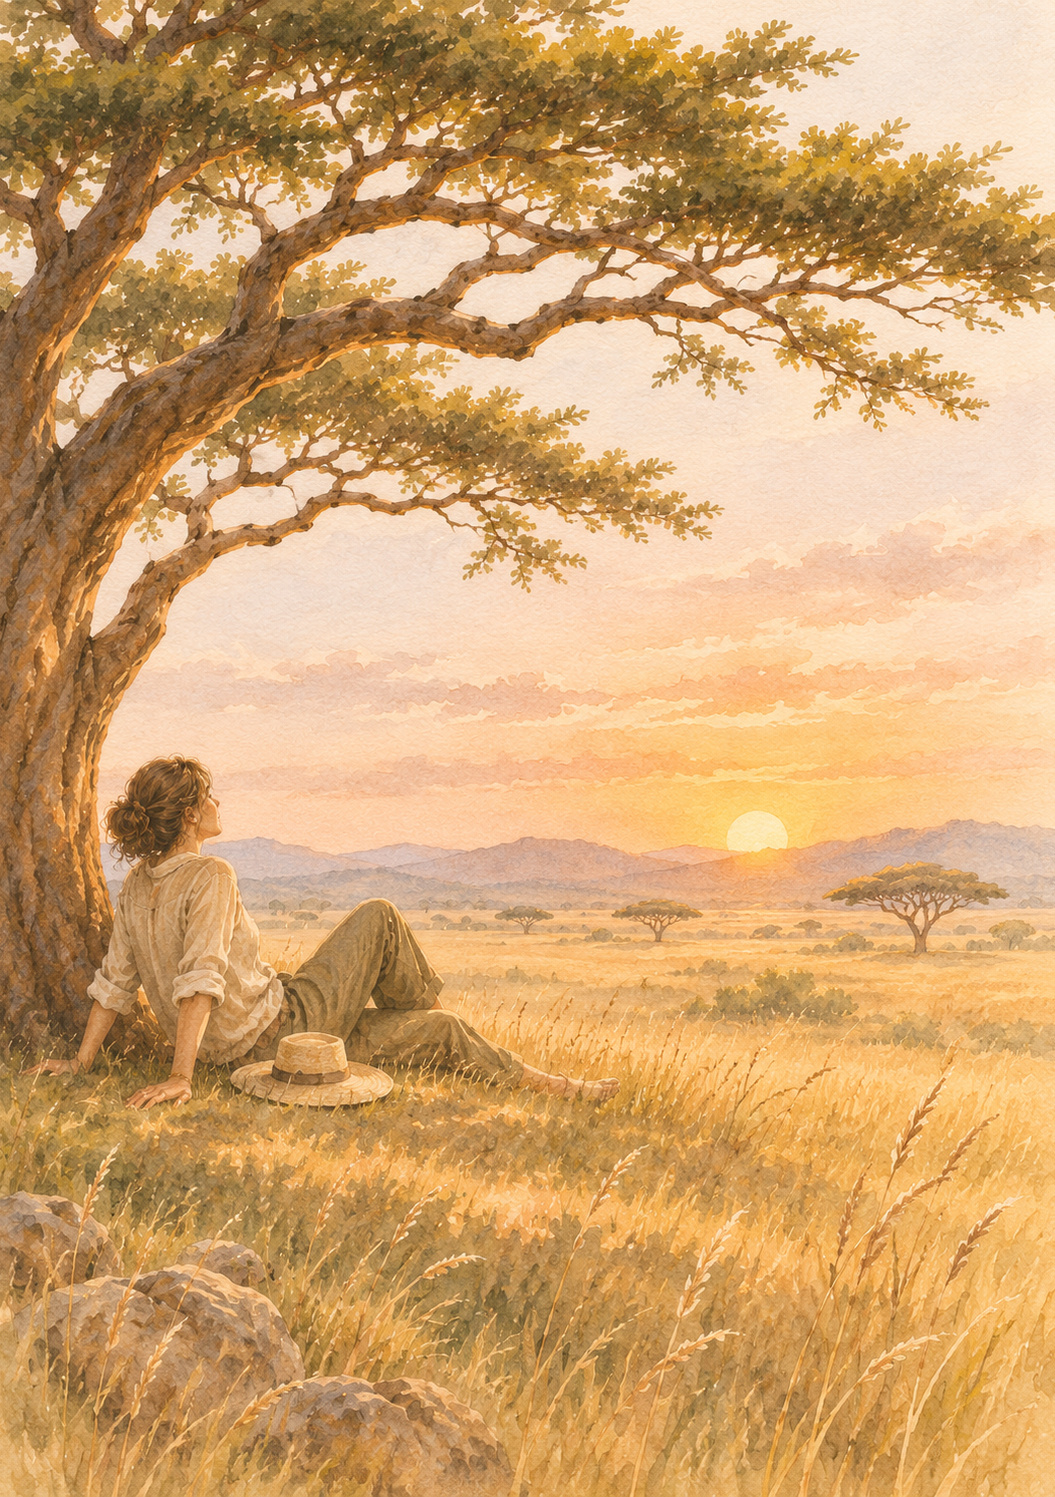
\includegraphics[width=\paperwidth,height=\paperheight]{assets/illustrations/12_hakuna_matata.jpg}
\end{ArtFullPage}
